\chapter[Article publié ou sous presse]
        {Titre long en français d'un chapitre contenant un article publié ou sous presse}
         \label{chap:publie}
        
\begin{authorsArticle}   % dans l'ordre de la publication
	\begin{description}
		\item[\large nom 1] Affiliation
		\item[\large nom 2] Affiliation
		\item[\large ...] 
	\end{description}
\end{authorsArticle}
%\authorArticle{
%}

\begin{abstractArticle}
	Résumé de l'article en français (in english if the language of the thesis is english). Ce résumé peut être la traduction de l'\textit{abstract} de l'article s'il est en anglais.
\end{abstractArticle}
% resumeArticle{}

\begin{contributions}
	Décrivez dans cette section les contributions de l'article.
\end{contributions}
               
\begin{commentairesArticle}
	Décrivez dans cette section la part de chacun.e des auteur.e.s
\end{commentairesArticle}

%\cleardoublepage 

%\begin{abstractArticle}
%Abstract
%\end{abstractArticle}

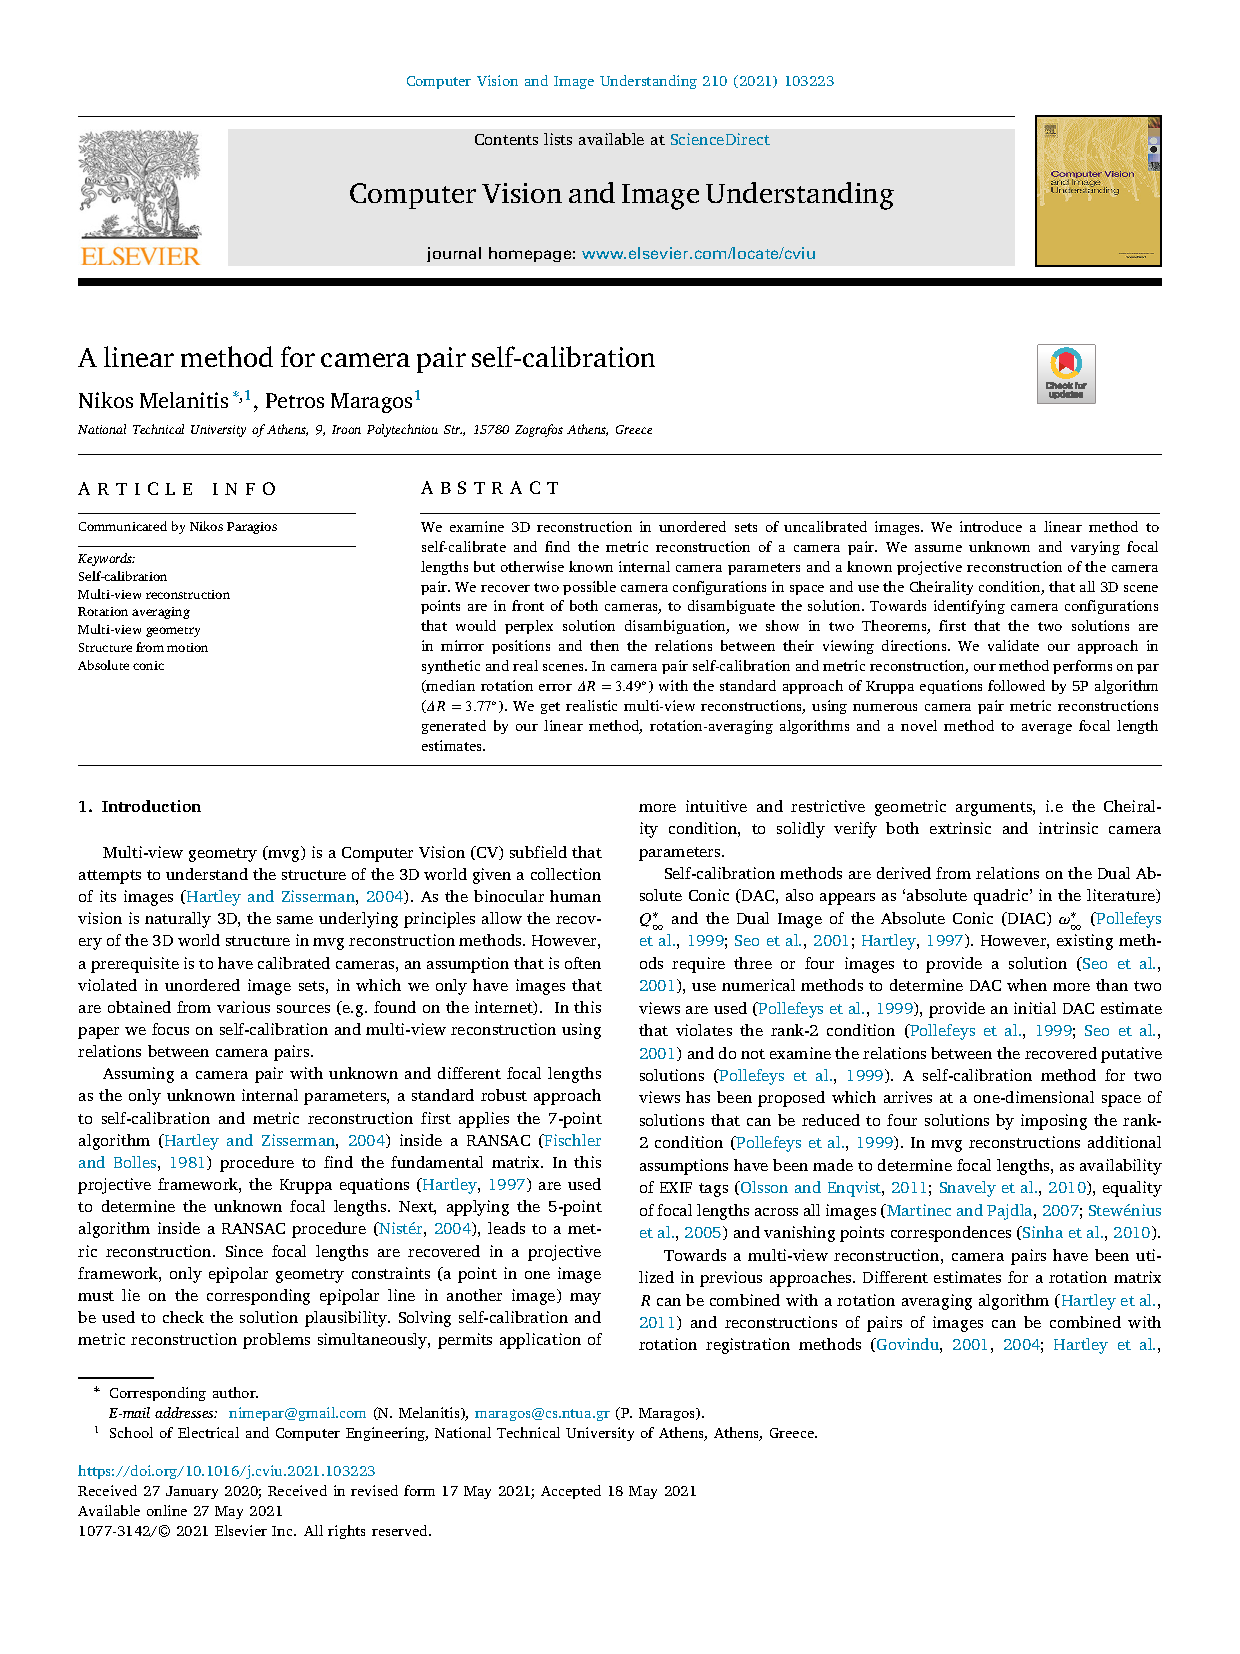
\includepdf[
	pages=-, % toutes les pages
	link=true, % permet de faire des hyperliens vers des pages en particulier
	linkname=article1, % pour les hyperliens, nom plus facile à manipuler
	addtotoc={
		1, section, 2, Titre original de l'article, sec:Article1,			%  item 1 Ne conserver que cet item dans le niveau  "section"
		2, subsection, 2, Background and related work, sec:AAA,    % item 2, page 2
		3, subsubsection, 4, A method for metric, sec:CCC,					% entree 3 non dans la TdM car on ne conserve que les étages 1 et 2
		4, subsection, 2, Recovering the solutions, subsec:BBB}	 % entree 4, page 4
]
{contenu/article.pdf} % nom et emplacement du fichier

%%%%%%%%%%%%%%%%%%%%%%%%%%%%%%%%%%%%%
% format de l'option addtotoc pour ajouter des éléments de l'article dans la table des matières. Ne pas en abuser.
%addtotoc={⟨page number ⟩,⟨section ⟩,⟨level ⟩,⟨heading ⟩,⟨label ⟩}
%⟨page number ⟩: Page number of the inserted page.
%⟨section⟩: LATEX sectioning name – e.g., section, subsection, . . .
%⟨level ⟩: Number, denoting depth of section – e.g., 1 for section level, 2 for subsection level, . . . si le niveau est plus grand que la prof. de la TOC (par défaut 2), aucun numéro n'apparait
%⟨heading⟩: Title inserted in the table of contents.
%⟨label ⟩: Name of the label. This label can be referred to with \ref and \pageref.

\section{Conclusion ou sections supplémentaires}

Rien n'empêche de conclure à part dans la langue principale du document. 

Possible de renvoyer à une page de l'article inséré à partir de n'importe où dans le document, comme suit :
\hyperlink{article1.5}{page 5} de l'article.

\Secref{CCC}.

Page \pageref{subsec:BBB}